\documentclass[12pt,a4paper]{article}

% Mathematics
\usepackage{amsmath,amssymb}
\usepackage{bbm}
\usepackage{slashed}

% Graphics
\usepackage{graphicx}
\usepackage{epsfig}
\usepackage{epstopdf}

% Tables and page layout
\usepackage{multirow}
\usepackage{placeins}
\setlength{\parskip}{10pt}

% Text formatting and URLs
\usepackage[normalem]{ulem}
\usepackage{url}

% Colors and cross-document citations
\usepackage[dvipsnames]{xcolor}
\usepackage{xcite}
\externalcitedocument{main-v6}

% Hyperlinks (load near the end)
\usepackage[
    colorlinks=true,
    citecolor=purple,
    linkcolor=blue
]{hyperref}

\begin{document}

\subsection*{Response to the Referee}

\noindent Dear Editor,

This paper considers an anomaly-free, renormalizable model of an additional Abelian
gauge boson \(A'\) with chiral couplings to muons and taus. In this model, vector-like
leptons and a scalar field \(S\) are introduced to construct the ultraviolet completion
of the axial \(U_A(1)_{L_{\mu-\tau}}\) gauge theory. The phenomenology of the \(A'\) in
the axial limit is studied, and the relevant experimental constraints are discussed.
The muon-collider calculation is presented only as an illustrative future-test example, not as a comprehensive collider study or a projected exclusion reach.

The referee summarizes our work as follows:

\begin{quote}
\itshape
The authors construct an anomaly-free, renormalizable model in which an additional Abelian gauge field \(A'\) has chiral couplings to muons and taus. This model realizes a limit where the \(A'\) coupling to the \(\mu-\tau\) current is axial. The second goal of the paper is to examine the phenomenology of this model in the axial limit.

The paper presents results that are useful for the model building community. However, I have some significant reservations about key points that either should be included or otherwise justified in being excluded from the manuscript. These are explained below. Revisions for these major points (even if only to clarify why they are not issues) are required before the paper is at the level of a PRD manuscript.
\end{quote}

We thank the referee for recognizing the model-building result and for identifying places where the relation between the UV construction and the effective-current phenomenology needs to be made clearer. In the replies below, we state which existing results or additional checks address each concern and distinguish those results from conclusions that would require a broader UV-model analysis.

\medskip
\noindent {\bf Major Points 1)}. \begin{quote}\itshape
Phenomenology of the \(S\) scalar. The second half of the paper reviews a set of experimental bounds on only an effective theory of the \(A'\) axially coupled to the \(L_{\mu-\tau}\) current. This leaves a major gap between these two parts of the paper: the authors show that their UV theory requires a scalar \(S\) that cannot be arbitrarily decoupled from the low-energy dynamics, e.g. from Eq. (34) which states that \(m_S^2 < 4\pi\left(m_{A'}/(2g_X)\right)^2\).\end{quote}

\noindent {\bf Reply.}
We agree with the referee's central point: \(S\) is a required degree of freedom in the UV construction and cannot be declared phenomenologically irrelevant simply because Fig.~2 focuses on \(A'\). Our choice is to keep the paper's main question—the axial-current phenomenology of \(A'\)—while making explicit which scalar constraints already bear on the model and which require a separate collider interpretation.

For the small-portal reference benchmark used in Fig.~2, the mass relations are
\[
m_{A'}=2g_Xv_s,\qquad m_s^2=2\lambda_Sv_s^2,
\qquad
\lambda_S=\frac{2g_X^2m_s^2}{m_{A'}^2}.
\]
Thus, imposing \(\lambda_S\leq\lambda_S^{\max}\) gives the conditional theoretical bound
\[
m_s\leq\sqrt{2\lambda_S^{\max}}\,v_s
=\sqrt{\frac{\lambda_S^{\max}}{2}}\frac{m_{A'}}{g_X}.
\]
For \(\lambda_S^{\max}=4\pi\), this is \(m_s\leq\sqrt{8\pi}\,v_s\); the reference choice \(m_s=10\,\mathrm{GeV}\) then requires \(v_s\gtrsim1.995\,\mathrm{GeV}\). These relations explain the scalar-sector consistency condition used alongside the \(A'\) benchmark. They are not experimental exclusions.

The scalar contribution to \((g-2)_\mu\) is also included in the paper's scalar analysis. For the reference \(m_s\gtrsim10\,\mathrm{GeV}\) benchmark, the scalar term in Eq.~\eqref{eq:gminus2-total} is below \(0.2\%\) of the pure-axial \(A'\) contribution, which is why the Fig.~2 contour uses the scalar-decoupling limit. For a lighter \(S\), the combined \(A'+S\) correction can change and can approach a cancellation region; the same contour should therefore not be read as a constraint for arbitrary \(m_s\).

To put the relevant evidence in the reply itself, we reproduce selected, non-exhaustive low-mass limits in the scalar-coupling parameterization. Direct entries constrain \(y_{s\mu\mu}\), while fifth-force tests require matching loop-induced couplings to ordinary matter. For the ultralight binary-pulsar result, we use Liu and Tang's scalar-mediator analysis, including its reported sensitivity interval and best-sensitivity point~\cite{Liu:2025zuz}; we do not transfer the \(L_\mu-L_\tau\) vector-mediator limit in Ref.~\cite{Dror:2019uea} as a direct scalar-Yukawa bound:
\begin{center}
\small
\begin{tabular}{p{0.28\linewidth}p{0.39\linewidth}p{0.20\linewidth}}
\hline
Scalar-mass range & Published constraint & Approximate bound / applicability for \(y_{s\mu\mu}\)\\
\hline
\(10^{-17}\,\mathrm{eV}\lesssim m_s\lesssim2\times10^{-15}\,\mathrm{eV}\) & Binary-pulsar periastron advance (95\% CL), ultralight scalar~\cite{Liu:2025zuz} & \(\mathcal{O}(10^{-21})\) at the best-sensitivity point \(m_s\simeq4\times10^{-16}\,\mathrm{eV}\)\\
\(m_s\lesssim10^{-2}\,\mathrm{eV}\) & Fifth-force tests via loop-induced ordinary-matter couplings~\cite{Fiorillo:2026wso,Hoskins:1985tn,Kapner:2006si,Blakemore:2021zna} & No universal direct \(y_{s\mu\mu}\) limit quoted\\
\(m_s\lesssim1\,\mathrm{keV}\) & Neutron-star cooling~\cite{Fiorillo:2026wso} & \(\lesssim7.4\times10^{-14}\)\\
\(m_s\lesssim1\,\mathrm{keV}\) & SN~1987A cooling (conservative cold-SN model)~\cite{Fiorillo:2026wso,Caputo:2021rux} & \(\lesssim4.2\times10^{-9}\)\\
\(100\,\mathrm{keV}\lesssim m_s\lesssim\mathcal{O}(10)\,\mathrm{MeV}\) & Diffuse supernova \(\gamma\)-ray background~\cite{Caputo:2021rux} & \(\lesssim4\times10^{-11}\)\\
\hline
\end{tabular}
\end{center}
These are approximate, source-dependent constraints, not a combined exclusion band. They establish that the low-mass scalar is not being assumed unconstrained: the cooling limits use the scalar results in Fiorillo et al.'s Table~1 for the stated regime~\cite{Fiorillo:2026wso}, while the diffuse-supernova-\(\gamma\)-ray result applies above approximately \(100\,\mathrm{keV}\) in Caputo et al.'s reference setup~\cite{Caputo:2021rux}. The fifth-force result depends on loop-induced couplings to ordinary matter and must be matched to this UV benchmark. The purpose of the table is to identify the applicable source constraints and their coupling definitions, not to turn them into a universal \(g_X\) exclusion.

\[
g_X<\frac{y_{\max}m_{A'}}{2m_\mu}.
\]
This conversion is conditional on the scalar--muon Yukawa normalization and the benchmark assumptions stated above. The low-mass entries should not be extrapolated to the \(m_s\geq10\,\mathrm{GeV}\) reference benchmark used for Fig.~2; collider-mass constraints require a separate interpretation, as discussed next.

\begin{figure}[htbp]
\centering
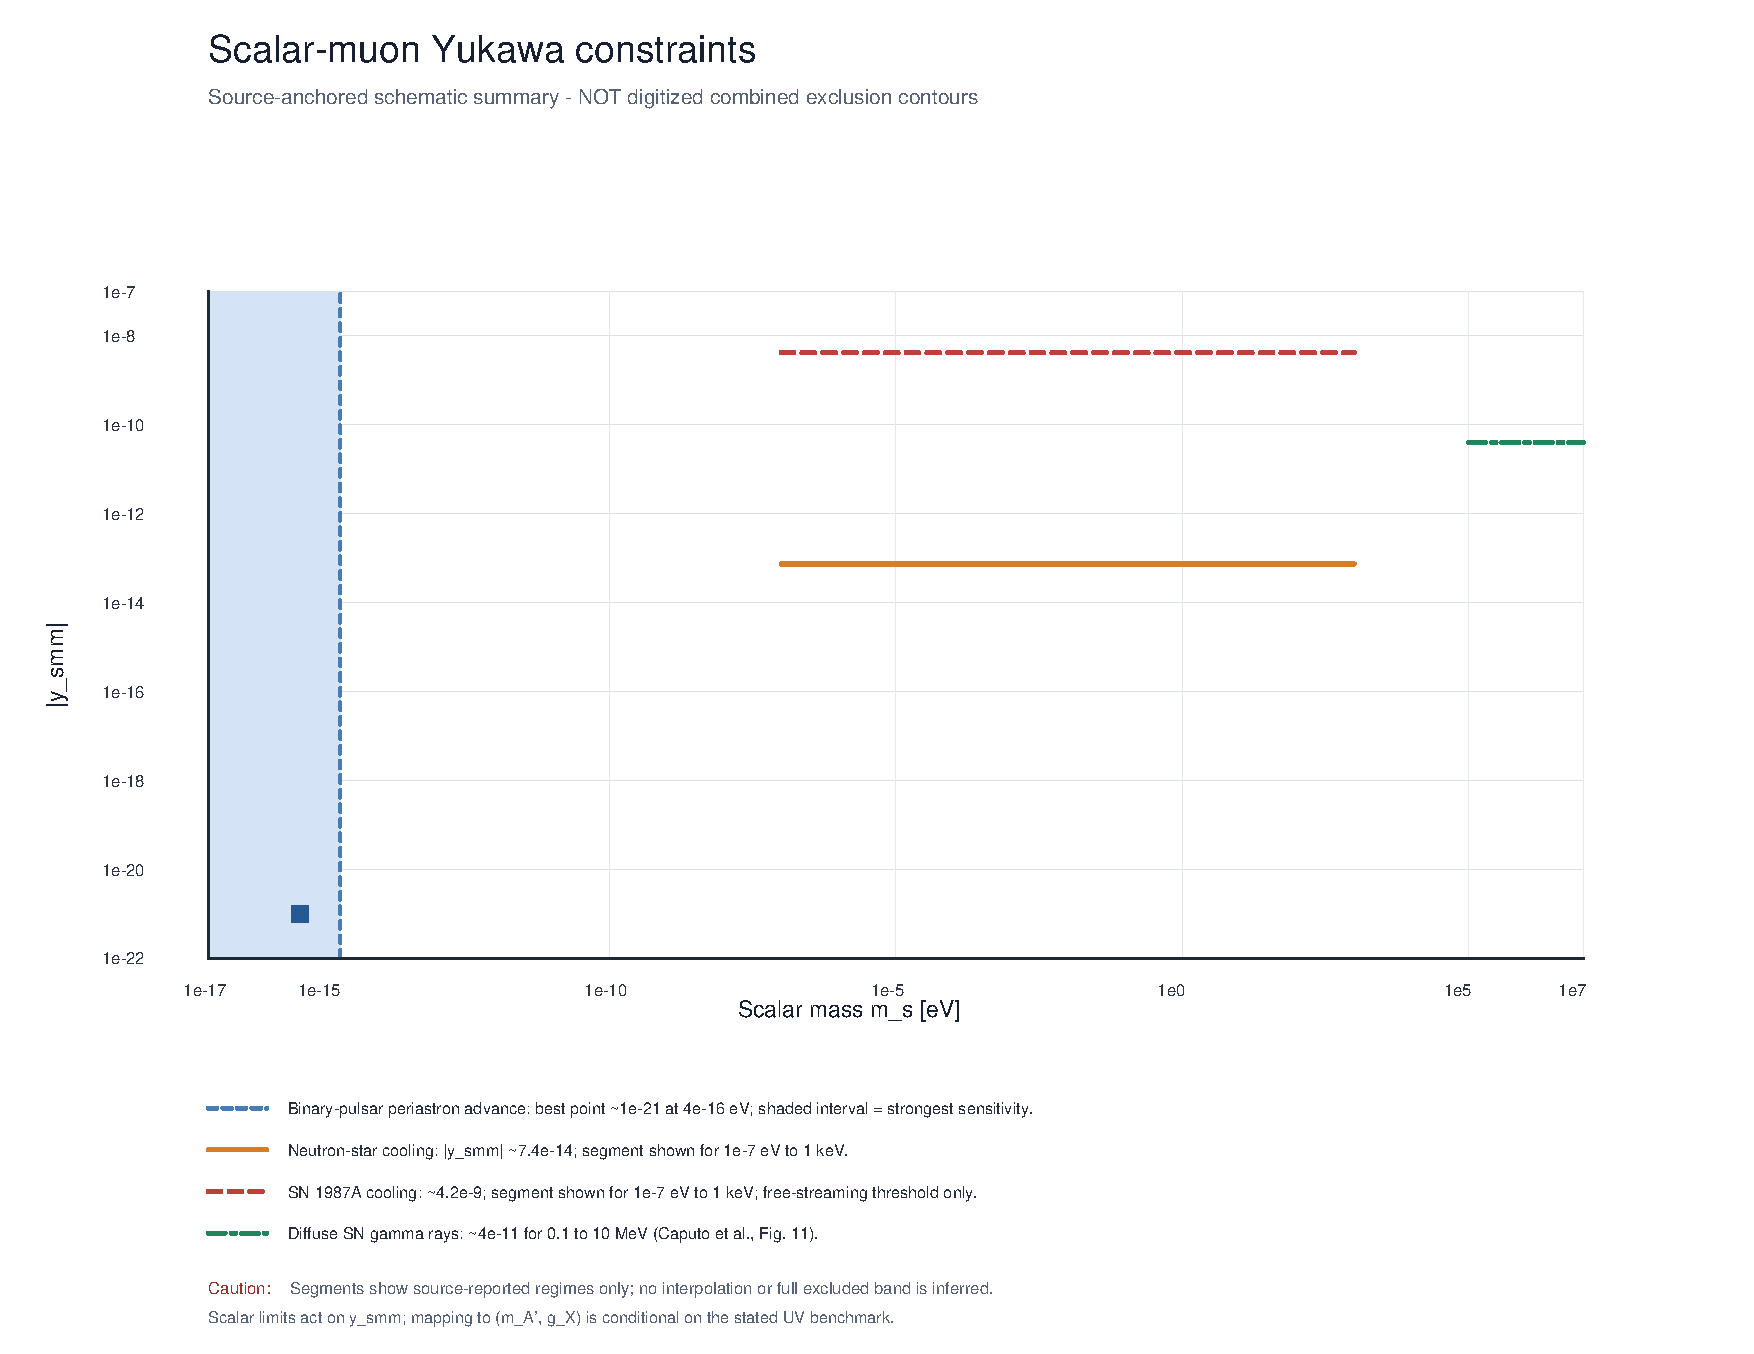
\includegraphics[width=0.96\linewidth]{审稿意见-gpt/当前执行/论文修改与一致性核查/2026-10-27/scalar_coupling_constraints_2026-10-28.pdf}
\caption{Source-anchored summary of selected constraints on the scalar--muon Yukawa coupling \(y_{s\mu\mu}\). The horizontal segments show only source-reported approximate limits in the indicated mass regimes; the binary-pulsar marker gives the published 95\% CL best-sensitivity point and the shaded interval indicates the mass range where that analysis reports its strongest sensitivity. The best-sensitivity value is not treated as a uniform limit across the shaded interval, and the figure is not a digitized combined exclusion contour. In particular, the SN~1987A line shows the free-streaming cooling threshold only and does not represent the full trapping/explosion-energy exclusion. These scalar constraints are not direct limits on the pure-axial \(A'\) current; the UV translation is conditional on \(y_{s\mu\mu}=2g_Xm_\mu/m_{A'}\) and a fixed scalar-mass benchmark within each source's applicability range; the light-scalar bounds shown here do not apply to the \(m_s\gtrsim10\,\mathrm{GeV}\) reference benchmark used for Fig.~2~\cite{Liu:2025zuz,Fiorillo:2026wso,Caputo:2021rux}.}
\label{fig:scalar-muon-constraints-response}
\end{figure}

\medskip
\noindent {\bf Major Points 1.1)}. \begin{quote}\itshape
It is thus an odd choice to exclude the scalar from the phenomenology of the effective theory: if the \(S\) is unavoidable at phenomenologically relevant scales, shouldn't one of the main points of the paper be that the only known UV completion of an axial \(L_{\mu-\tau}\) gauge boson has a prediction for a scalar particle in a mass range that can be probed by colliders?\end{quote}

\noindent {\bf Reply.}
Yes: \(S\) is a prediction of the UV completion, and collider searches can in principle test it. We do not omit \(S\) from the UV model; we separate its phenomenology from Fig.~2 because that figure presents constraints on the \(A'\) effective current, whereas scalar searches depend on additional quantities that are not fixed by the two plotted parameters alone.

The existing singlet--Higgs literature establishes how Higgs signal strengths and direct scalar searches depend on the portal mixing and scalar mass~\cite{Robens:2015singlet,Robens:2020twoSinglets,Boiarska:2019scalarPortal}. Dedicated leptophilic-scalar searches at BaBar, Belle and Belle~II also cover relevant production channels and mass ranges~\cite{BaBar:2020jma,Belle:2022gbl,Belle-II:2024wtd,Belle-II:2023ydz}. For example, the Belle~II four-muon search includes a muonphilic spin-0 interpretation over approximately \(0.212\text{--}9.0\,\mathrm{GeV}\), while the \(\mu^+\mu^-\tau^+\tau^-\) search includes a Higgs-like leptophilic interpretation over approximately \(3.6\text{--}10\,\mathrm{GeV}\). These searches establish relevant coverage, but they are not interchangeable: their production modes, coupling normalizations, decay selections and acceptances differ.

The point of citing these results is to identify where the radial scalar can be searched for, not to claim that the published limits automatically exclude it in our UV model. A model-specific interpretation must use the matched scalar coupling and portal mixing, and account for branching fractions, widths, lifetime and acceptance, including \(s\to A'A'\) when open. The present response therefore connects the scalar to the relevant existing searches without presenting an unperformed global scalar-collider recast as a result.

\medskip
\noindent {\bf Major Points 1.2)}. \begin{quote}\itshape
What is the range of phenomenologically allowed \(S\) mass including perturbativity limits on \(\lambda\) and a motivated range of \(m_{A'}\) and \(g_X\). For example: perhaps the authors imagine a range of \(m_{A'}\) below some benchmark mass where certain experimental constraints on \(g_X\) become very strong. Then with that set of constraints (which should be stated clearly, see minor point \#1 below), one may give a range of \(m_S\) and comment on the experimental constraints.\end{quote}

\noindent {\bf Reply.}
The allowed \(m_s\) range is conditional on the chosen \((m_{A'},g_X)\) point and on which scalar constraints apply; it is not a single interval that can be read off from the \(A'\) contours. The referee's suggested comparison is the right way to organize the question: first impose the UV consistency condition, then apply the experimental limits using the scalar coupling and decay assumptions relevant to each search.

In the one-VEV benchmark, \(v_s=m_{A'}/(2g_X)\) and
\[
\lambda_S=\frac{m_s^2}{2v_s^2}
=\frac{2g_X^2m_s^2}{m_{A'}^2}.
\]
A specified perturbativity criterion \(\lambda_S\leq\lambda_S^{\max}\) gives
\[
m_s\leq\sqrt{2\lambda_S^{\max}}\,v_s.
\]
For \(\lambda_S^{\max}=4\pi\), this is \(m_s\leq\sqrt{8\pi}\,v_s\). If the scalar-suppressed reference benchmark \(m_s\geq10\,\mathrm{GeV}\) is adopted, it requires \(v_s\gtrsim1.995\,\mathrm{GeV}\), equivalently \(m_{A'}\gtrsim(3.99\,\mathrm{GeV})g_X\). This is the conditional scalar-sector consistency boundary represented by the dashed line, not an experimental lower bound on \(m_s\).

The scalar limits summarized under Major Point~1 constrain \(y_{s\mu\mu}\) or source-specific induced matter couplings; the collider searches under Major Point~1.1 require a model-matched interpretation. Taken together, these results show how the theoretical and experimental conditions enter, but they do not establish a global phenomenologically allowed \(m_s\) interval for the full UV parameter space. We therefore state the conditional mass relation and the source-specific constraints rather than assigning a single allowed interval unsupported by a consistent joint analysis.

\medskip
\noindent {\bf Major Points 1.3)}. \begin{quote}\itshape
Above (34): the authors ``assume negligible Higgs-portal mixing.'' Is this interaction not generated at loop level? It seems that \(S\)-\(h\) mixing cannot be avoided due to \(\mu\) and \(\tau\) loops. In turn, this seems like it would lead to strong experimental bounds on the UV completion. In fact, once there is mixing, is there not a resonance where the mixing becomes large as \(m_S\to m_h\)? It would be useful to quantify the size of this mixing over the allowed range of \(m_S\). Existing Higgs measurements may set the strongest bounds on the UV completion. If these bounds are obviously negligible (though again, I expect this to be strongly constrained as \(m_S\to m_h\)), then the authors should present this as the justification for ignoring \(m_S\) in the low-energy theory. (Though I am still skeptical that the \(S\) can be ignored since it cannot formally decouple.)\end{quote}

\noindent {\bf Reply.}
The referee is correct that the portal operator \((H^\dagger H)(S^\dagger S)\) is allowed by the gauge symmetry, so a negligible portal is not a symmetry-protected prediction. To address the loop concern quantitatively, we evaluated the leading VLL threshold and the finite-momentum off-diagonal self-energy under an explicit matching condition, \(\lambda_{HS}^{\mathrm{EFT}}(M_E)=0\). This is a specified small-portal benchmark; it requires a nonzero UV portal, \(\lambda_{HS}^{\mathrm{UV}}=-\Delta\lambda_{HS}^{E}\), and is not independent of the renormalized boundary condition.

At zero momentum, the VLL threshold in the potential convention used here is
\[
\Delta\lambda_{HS}^{E}
=-\frac{1}{8\pi^2}\sum_{\ell=\mu,\tau}|y_\ell|^2|\lambda_\ell|^2.
\]
For \(M_E=20\,\mathrm{TeV}\) and \(\theta_{\mu L}=\theta_{\tau L}=10^{-2}\), the two illustrative benchmarks give \(\Delta\lambda_{HS}^{E}\simeq-0.2108\) at \((m_{A'},g_X,v_s)=(10\,\mathrm{GeV},0.0705,70.9\,\mathrm{GeV})\), and \(-0.01067\) at \((63\,\mathrm{GeV},0.1,315\,\mathrm{GeV})\). This shows why setting the UV portal to zero and setting the matched EFT portal to zero are different assumptions.

We also evaluated the leading charged-lepton/VLL contribution to \(\Pi_{hs}(p^2)\) using the full \(2\times2\) mass-eigenstate matrices, including light--light, light--heavy, heavy--light and heavy--heavy internal states. In the zero-tree-level-mixing setup there is no tree-level \(sWW\) or \(s\bar t t\) vertex, so direct \(W\)- or top-quark diagrams do not contribute at this order. At \(p^2=m_h^2\), the matched self-energy is
\[
\Pi_{hs}^{\mathrm{matched}}(m_h^2)
\simeq(-0.4133-0.1132i)\,\mathrm{GeV}^2
\]
for the first benchmark above, and
\[
\Pi_{hs}^{\mathrm{matched}}(m_h^2)
\simeq(-0.09300-0.02547i)\,\mathrm{GeV}^2
\]
for the second.

These results answer the loop-generation question: the mixing contribution is calculable and depends on the matching condition and benchmark. They also show why one cannot dismiss the near-degenerate case by quoting a generic small-mixing estimate. At \(m_s=m_h=125.25\,\mathrm{GeV}\), the width-regulated diagnostic \(2|\Pi_{hs}/(a-b)|\) is about \(9.1\times10^{-4}\) when \(s\to A'A'\) is open with \(\Gamma_s\simeq3.75\,\mathrm{GeV}\), but reaches about \(0.394\) at exact degeneracy in the closed-channel benchmark with \(\Gamma_s\simeq0.159\,\mathrm{MeV}\). In the latter case the fixed-self-energy diagnostic exceeds \(0.1\) only in a narrow band around \(m_h\), approximately \(7.5\,\mathrm{MeV}\) on either side, where \(a=m_h^2-i m_h\Gamma_h\) and \(b=m_s^2-i m_s\Gamma_s\).

The last quantity is a diagnostic, not a self-consistent two-pole solution or a Higgs signal-strength exclusion. It identifies where the small-mixing approximation needs special care; it does not establish a global Higgs constraint or classify the near-degenerate UV parameter space as allowed or excluded. The scalar remains part of the UV model, while Fig.~2 retains its stated role as the \(A'\) effective-current benchmark.

\medskip
\noindent {\bf Major Points 2)}. \begin{quote}\itshape
Motivating the range of effective theory parameters. To further aid in the comparison between the UV theory and the two-parameter low-energy theory, it would be useful to explicitly state in one place (perhaps in a table or a figure like Fig. 2) the range of the effective model parameters that are feasible. The main phenomenological results are in Fig. 2, but it was not clear why this range of couplings and \(A'\) masses were chosen: are values outside this range not allowed? What, if anything, does the perturbativity of the UV theory impose on the effective parameters?\end{quote}

\noindent {\bf Reply.}
The window in Fig.~2 is chosen to compare the complementary experimental regimes used in this paper on a common \((m_{A'},g_X)\) plane; it is not a claim that the endpoints delimit the full allowed parameter space. The displayed ranges are
\[
10^{-3}\,\mathrm{GeV}\leq m_{A'}\leq10^2\,\mathrm{GeV},
\qquad
10^{-6}\leq g_X\leq10^{-1}.
\]
The mass interval spans low-energy precision tests, pion and kaon decays, beam-dump searches, neutrino trident production, visible-resonance searches at \(B\) factories and higher-energy collider searches. For example, PIENU is kinematically sensitive below \(m_{\pi^+}-m_\mu\simeq33.9\,\mathrm{MeV}\)~\cite{PIENU:2021clt,Altmannshofer:2026opc}, NA62 reaches below \(m_{K^+}-m_\mu\simeq388\,\mathrm{MeV}\) in the channel shown as an indicative recast~\cite{NA62:2021bji}, and BaBar/Belle~II and CMS cover complementary higher-mass visible-resonance regimes~\cite{BaBar:2016sci,Belle-II:2024wtd,CMS:2018yxg}. These searches do not provide uniform coverage at every mass.

The lower endpoint \(1\,\mathrm{MeV}\) keeps the low-energy precision and terrestrial-search regimes compared in this paper visible on the same plot. Extending below it is possible, but would require a dedicated treatment of the additional very-low-energy and stellar constraints; the plotted endpoint itself is not a lower mass bound. The upper endpoint \(100\,\mathrm{GeV}\) is a presentation choice covering the higher-mass terrestrial searches considered here, not an experimental upper limit or a theoretical cutoff. Likewise, \(10^{-6}\) and \(0.1\) are scan endpoints, not universal lower and upper bounds on \(g_X\). Although \(g_X=0.1\) is below the usual gauge-coupling perturbativity criterion, perturbativity alone does not select \(0.1\) as a maximum.

The UV consistency condition relevant to the dashed line comes from the scalar sector. In the one-VEV benchmark,
\[
v_s=\frac{m_{A'}}{2g_X},\qquad
\lambda_S=\frac{m_s^2}{2v_s^2}
=\frac{2g_X^2m_s^2}{m_{A'}^2}.
\]
Thus \(\lambda_S\leq\lambda_S^{\max}\) implies \(m_s\leq\sqrt{2\lambda_S^{\max}}\,v_s\). For \(\lambda_S^{\max}=4\pi\) and the reference choice \(m_s\geq10\,\mathrm{GeV}\), this gives
\[
v_s\gtrsim1.995\,\mathrm{GeV},
\qquad
m_{A'}\gtrsim(3.99\,\mathrm{GeV})g_X.
\]
The dashed line therefore marks the boundary of that specified scalar benchmark. It is not a universal exclusion of points below the line or a global UV-viability contour.

The plotted information should consequently be read in three steps: a displayed contour excludes only under the assumptions of its source analysis; a point not excluded by those contours is not automatically a viable point of the full UV model; and a point below the dashed line fails the chosen \(m_s\geq10\,\mathrm{GeV}\), \(\lambda_S\leq4\pi\) benchmark, not every possible scalar-sector realization. This is the intended comparison between the effective-current results and the UV consistency condition.

\medskip
\noindent {\bf Major Points 3)}.

\begin{quote}\itshape
Are neutrino oscillations possible? The Standard Model is defined with only left-handed neutrinos because of the possibility that neutrinos are their own antiparticle. In such a case neutrino masses are generated through, e.g. through the Weinberg operator.
\end{quote}

\medskip
\noindent {\bf Reply to Point 3.1}

\begin{quote}\itshape
In this model, \(U_A(1)_{L_{\mu-\tau}}\) invariance allows Weinberg operators for each generation. However, it appears that both the Yukawa matrices and neutrino masses must be aligned and therefore a non-trivial PMNS matrix does not appear to be possible.
\end{quote}

\noindent {\bf Reply.}
The minimal construction can accommodate some symmetry-allowed neutrino mass terms, but it does not reproduce the observed PMNS matrix. We checked the operator-selection rules for the charge assignment
\[
Q'(L_e,L_\mu,L_\tau)=(0,+Q_\ell,-Q_\ell),\qquad
Q'(H)=0,\qquad Q'(S)=2Q_\ell.
\]
At dimension five, \((L_eH)(L_eH)\) and \((L_\mu H)(L_\tau H)\) are allowed. The \(\mu\mu\) and \(\tau\tau\) entries first arise with one \(S^\dagger\) or \(S\) insertion, respectively, at dimension six. The \(e\mu\) and \(e\tau\) entries remain forbidden because insertions of \(S\) or \(S^\dagger\) change the charge only by even multiples of \(Q_\ell\).

The resulting neutrino mass matrix has the block form
\[
M_\nu=
\begin{pmatrix}
A&0&0\\
0&B\varepsilon&C\\
0&C&D\varepsilon
\end{pmatrix},
\qquad \varepsilon\sim v_s/\Lambda,
\]
and the charged-lepton Yukawa matrix has the same \(\{e\}\oplus\{\mu,\tau\}\) block structure. Consequently, up to mass-eigenstate ordering and phase conventions,
\[
U_{\rm PMNS}=\operatorname{diag}(1,U_{23}).
\]
A nontrivial \(\mu\)--\(\tau\) rotation is possible, but the electron-flavor admixtures required by the observed nonzero \(\theta_{12}\) and \(\theta_{13}\) are absent. Thus the symmetry-allowed EFT operators show what the minimal charge assignment permits; they do not make the minimal renormalizable UV Lagrangian a complete neutrino-mass mechanism or establish the coefficients of those operators.

\medskip
\noindent {\bf Reply to Point 3.2}

\begin{quote}\itshape
Perhaps a full model would require right-handed neutrinos. These would now be charged under \(U_A(1)_{L_{\mu-\tau}}\), which likely means the second and third generation must appear as vectorlike combinations. However, it seems to me that mixing between generations is prohibited by \(U_A(1)_{L_{\mu-\tau}}\).
\end{quote}

\noindent {\bf Reply.}
Right-handed neutrinos alone do not remove the obstruction if the same residual \(Z_2\) selection rule is preserved. The Dirac and Majorana mass matrices then remain block diagonal between the electron-flavor sector and the \(\mu\)--\(\tau\) sector, so the seesaw relation \(M_\nu=-m_D M_R^{-1}m_D^T\) does not generate the missing electron-flavor mixing.

Gauged \(L_\mu-L_\tau\) constructions with additional neutrino-sector structure have been studied, for example, by Heeck and Rodejohann~\cite{Heeck:2011wj} and Asai, Hamaguchi and Nagata~\cite{Asai:2017ryy}. Those models illustrate that extensions are possible, but their field content and charge assignments are not identical to ours. An additional scalar with an odd \(U_A(1)\) charge and a nonzero vacuum expectation value could break the residual selection rule; that would be a nonminimal extension, not a solution within the present field content. We therefore retain the anomaly-free gauge and charged-lepton construction and do not claim that it explains the full neutrino mass spectrum or PMNS matrix.

\medskip
\noindent {\bf Overall response to Major Point 3.}

\begin{quote}\itshape
Thus it is not obvious to me how neutrino oscillations can be included in this framework. If there is a simple solution, the authors should include it. If there is a known less-simple solution in the literature, the authors should cite this. Otherwise, at best this will be a confusing point. At worst, it would make the construction inconsistent with neutrino oscillation experiments.
\end{quote}

\noindent {\bf Reply.}
The direct answer is that the minimal construction does not reproduce the observed PMNS matrix. Its allowed mass terms can give a \(\mu\)--\(\tau\) sector, but the electron--muon and electron--tau entries are forbidden by the residual symmetry. A complete oscillation model would require additional structure that changes this selection rule; adding right-handed neutrinos without doing so is insufficient. We keep the present paper's claims to the anomaly-free gauge/charged-lepton construction and its axial-vector phenomenology, rather than adding a new neutrino sector solely for this revision.

\medskip
\noindent {\bf 4)}.
\begin{quote}\itshape
Is this the full set of experimental constraints? The second half of the manuscript presents a set of experimental bounds on the two-parameter effective \(A'\) model. It is not obvious if this is the full set of constraints on the model. (See also point \#1 above: I would have liked to see a section discussing the bounds on the \(S\) within this model since it cannot be decoupled.) The following experimental bounds seem like they could be relevant. It would be helpful to either include them or justify why they are subdominant to the experiments presented.
\end{quote}

\noindent {\bf Reply.}
No: Fig.~2 is not intended to be an exhaustive list of every constraint on every realization of the UV model. It presents the constraints applied to the specified two-parameter, pure-axial effective-current benchmark. To address the referee's concrete suggestions, we have checked the scalar constraints separately (Major Point~1), estimated the loop-induced kinetic mixing, quantified the leading finite-vector effects in the observables evaluated, and identified which supernova contributions can be carried over because the neutrino couplings are unchanged. The following points state both the conclusion supported by each check and the conditions under which it applies; they do not turn the figure into a global UV fit.

\medskip
\noindent {\bf 4.1)}.
\begin{quote}\itshape
Neutrino oscillation observations. See point \#3 above. It appears that this model predicts a unit PMNS matrix, which is inconsistent with neutrino oscillations.
\end{quote}

\noindent {\bf Reply.}
The referee is right that the minimal model does not reproduce the observed PMNS matrix; however, the prediction is not necessarily the identity matrix. As shown under Major Point~3, the allowed mass matrices retain a \(\mu\)--\(\tau\) block but forbid the electron-flavor admixtures required by the observed nonzero \(\theta_{12}\) and \(\theta_{13}\). This is a limitation of the minimal construction, not a constraint addressed by the \(A'\) contours in Fig.~2.

\medskip
\noindent {\bf 4.2)}.
\begin{quote}\itshape
There is no quantitative estimate of the amount of kinetic mixing generated with the ``benchmark'' choices of \(\theta\leq10^{-2}\). The authors make the insightful point that kinetic mixing goes to zero in the axial limit, but because this limit is tied to the size of the mixing (the mass of the vectorlike leptons), for the above benchmark there is non-zero kinetic mixing. It would be useful to have parametric estimates of the amount of kinetic mixing one expects so that readers may compare to experimental bounds. One could invoke parametric expressions in the literature for the relevant loop diagrams.
\end{quote}

\noindent {\bf Reply.}
We have evaluated the requested parametric estimate in the equal-mixing benchmark \(\theta_{\mu R}=\theta_{\tau R}\equiv\theta_R\), with no additional bare low-energy kinetic-mixing term and the stated heavy-VLL matching condition. For degenerate heavy VLLs, the one-loop heavy threshold proportional to \(\ln(M_{E_\mu}^2/M_{E_\tau}^2)\) cancels; the residual contribution is generated by the light charged-lepton loops. Using the momentum-dependent expression of Hapitas, Tuckler and Zhang~\cite{Hapitas:2021kineticMixing},
\[
\epsilon_{\gamma A'}(q^2)=
-\frac{e\,g_X\sin^2\theta_R}{2\pi^2}
\int_0^1 dx\,x(1-x)
\log\!\left[
\frac{m_\tau^2-x(1-x)q^2-i0}
     {m_\mu^2-x(1-x)q^2-i0}
\right],
\]
we obtain at zero momentum
\[
|\epsilon_{\gamma A'}(0)|
=\frac{e|g_X|\sin^2\theta_R}{6\pi^2}
\ln\frac{m_\tau}{m_\mu}
\simeq1.44\times10^{-6}|g_X|
\quad(\theta_R=10^{-2}).
\]

For on-shell production, \(q^2=m_{A'}^2\), and the threshold dependence matters. Representative numerical values are
\[
\begin{array}{c|c}
m_{A'} & |\epsilon_{\gamma A'}(m_{A'}^2)|/|g_X|\\
\hline
10\,\mathrm{MeV} & 1.44\times10^{-6}\\
212\,\mathrm{MeV} & 2.12\times10^{-6}\\
1\,\mathrm{GeV} & 1.08\times10^{-6}\\
10\,\mathrm{GeV} & 5.47\times10^{-8}\\
100\,\mathrm{GeV} & 4.84\times10^{-10}
\end{array}
\]
The largest of these values occurs near the dimuon threshold and is about \(1.47\) times the zero-momentum magnitude, consistent with Wang and Zhang~\cite{Wang:2026supernova}. For \(g_X\leq0.1\), the corresponding largest \(|\epsilon_{\gamma A'}|\) is about \(2.1\times10^{-7}\).

This is the quantitative answer to the referee's question: kinetic mixing is nonzero for the finite-mixing benchmark, but its induced electron-current coupling is much smaller than the \(\mathcal O(10^{-4})\) sensitivity scale of the relevant NA64 missing-energy search below \(m_{A'}\lesssim0.35\,\mathrm{GeV}\)~\cite{NA64:2023lightDM}. It therefore does not set the leading laboratory constraint in the sub-GeV range where this comparison applies. The conclusion is conditional on equal mixing angles and the stated matching condition; it is not a universal prediction for arbitrary UV boundary conditions.

\medskip
\noindent {\bf 4.3)}.
\begin{quote}\itshape
Another way of reframing the above point: the bounds presented are in the pure axial limit. Since the authors present a UV model that only realizes the axial coupling in a decoupling limit, it would be useful to comment on possible experimental bounds on the small vector-like coupling in a model with non-infinite vectorlike fermion masses. If these bounds are always small compared to the axial bounds, this should be stated and justified. The importance of this point is as follows: often bounds are sensitive to the chiral structure of interactions. Sometimes a vector interaction is more tightly constrained than its axial counterpart. Since the authors focus on the phenomenology in the axial limit, one wants to make sure that any small-but-finite vector interaction isn't significant because the constraints on the coupling are orders-of-magnitude larger than the axial coupling.
\end{quote}

\noindent {\bf Reply.}
The relevant question is whether the finite vector component changes the constraints used for the axial benchmark. For \(|\theta_{\ell R}|\leq10^{-2}\), the mass-basis couplings satisfy
\[
\left|\frac{g_V^\ell}{g_A^\ell}\right|
=\tan^2\theta_{\ell R}\leq1.01\times10^{-4},
\]
so at \(g_X=0.1\), \(|g_V^\ell|\leq10^{-5}\), while the neutrino couplings remain \(g_{\nu_\mu}=+g_X\) and \(g_{\nu_\tau}=-g_X\).

We compared the leading vector and axial contributions in the two observables for which this correction is evaluated. For neutrino trident production, the ratio of the leading Standard-Model interference terms at the same momentum transfer is
\[
\left|\frac{C_V\delta C_V}{C_A\delta C_A}\right|
\sim\frac{C_V}{C_A}\tan^2\theta_{\mu R}
\lesssim2.0\times10^{-4},
\qquad C_V\simeq0.96,\quad C_A=\frac12,
\]
before the distinct finite-\(m_\mu\) response functions are included. For \((g-2)_\mu\),
\[
\left|\frac{\Delta a_\mu^V}{\Delta a_\mu^A}\right|
=\tan^4\theta_{\mu R}\frac{F_V(r)}{F_A(r)}
\lesssim2.1\times10^{-9},
\]
using \(F_V/F_A\leq0.20\) over the mass range considered. These comparisons show that the finite vector component does not materially change the leading trident-interference or \((g-2)_\mu\) result for the stated benchmark, even though vector and axial constraints are not interchangeable in general.

There is one relevant qualification for visible decays near threshold:
\[
\Gamma_V\propto(g_V^\mu)^2(1+2r_\mu)\sqrt{1-4r_\mu},\qquad
\Gamma_A\propto(g_A^\mu)^2(1-4r_\mu)^{3/2},
\quad r_\mu=\frac{m_\mu^2}{m_{A'}^2}.
\]
The vector-squared contribution is suppressed by \(\tan^4\theta_{\mu R}\leq10^{-8}\) away from threshold, but the stronger axial phase-space suppression can make it relevant to the branching fraction very close to \(2m_\mu\). We therefore apply the comparison to the observables and benchmark for which it was calculated, rather than claiming that every vector-sensitive search is unaffected.

\noindent {\bf 4.4)}.
\begin{quote}\itshape
Are stellar cooling bounds not relevant? See e.g. 2511.09619 for a recent paper on this. If they are not, then this is certainly worth justifying.
\end{quote}

\noindent {\bf Reply.}
Yes. Stellar constraints are relevant in the sub-GeV region, and we do not dismiss them. The referee-cited analysis is now published as JHEP 06 (2026) 155~\cite{Blinov:2025aha}; an updated calculation for the conventional vector \(L_\mu-L_\tau\) boson reports SN1987A sensitivity up to about \(300\,\mathrm{MeV}\) and low-energy-supernova sensitivity up to about \(600\,\mathrm{MeV}\) for the stated SFHo-18.8 profile~\cite{Wang:2026supernova}. These results provide useful reference scales, but the full vector-model exclusion curve cannot automatically be assigned to the axial model.

The part that can be compared directly is neutrino coalescence: at fixed \((m_{A'},g_X)\), our tree-level couplings \(g_{\nu_\mu}=+g_X\) and \(g_{\nu_\tau}=-g_X\) are unchanged, so neutrino-coalescence production and the invisible neutrino widths are unchanged. In the cited profile, this production channel dominates for \(m_{A'}\gtrsim10\,\mathrm{MeV}\); for \(10\,\mathrm{MeV}\lesssim m_{A'}<2m_\mu\), the published cooling result is therefore a relevant benchmark comparison.

The part that cannot be transferred without a model-specific calculation involves the charged-muon current. Semi-Compton production and inverse absorption depend on whether that current is vector or axial, and above \(2m_\mu\) the vector and axial dimuon widths have different threshold behavior. In the equal-mixing benchmark, the low-momentum kinetic mixing is \(|\epsilon_{\gamma A'}|/|g_X|\simeq1.4\times10^{-6}\), much smaller than the approximately \(1/70\) value in the conventional vector model. Thus the defensible conclusion is not that supernova bounds are irrelevant, but that the neutrino-coalescence component is a useful reference where it dominates, while the full vector-current supernova contour is not a model-independent exclusion of the axial construction.

\medskip
\noindent {\bf Minor Point 1)}. \begin{quote}\itshape
Range of parameters. The general construction of the model is clearly written, but it is difficult for the reader to envision the mass and coupling range that the authors are targeting. It would be very helpful if the authors decide on a range of \(m_{A'}\) and \(g_X\) of interest. For example: is there a range of masses where experimental or theoretical limits are less constraining? Is there some set of phenomenology that the authors seek to realize with a ``light'' \(A'\)? If so, they should define ``light.'' (See, e.g. the first word of the introduction, which is not defined with respect to any reference mass scale.)\end{quote}

\noindent {\bf Reply.}
The mass and coupling window shown in Fig.~2 is
\[
10^{-3}\,\mathrm{GeV}\leq m_{A'}\leq10^2\,\mathrm{GeV},
\qquad
10^{-6}\leq g_X\leq10^{-1}.
\]
It is chosen to display, on one plane, the low-energy precision, meson-decay/beam-dump, neutrino-trident, \(B\)-factory and higher-energy collider regimes discussed in the paper. We do not single out a mass interval as generically weakly constrained or define a separate phenomenological target through the word \emph{light}; the purpose is to compare the constraints across the stated range. The lower endpoint is not a lower mass bound, and the upper endpoint is not a theoretical cutoff; points outside the window are not excluded merely by being outside the plot. Likewise, the coupling endpoints are scan choices, not universal bounds. The adjective \emph{light} is not intended to define a separate quantitative regime, so the precise description is a neutral spin-one boson with the mass range stated explicitly.

\medskip
\noindent {\bf Minor Point 2)}.
\begin{quote}\itshape
Defining the pure-axial limit. Equation (12) gives the coupling of the \(A'\) to the mass-basis fields. It is here that the ``pure axial coupling'' limit is defined? i.e. \(\theta_{\mu R}\to0\)? If that is the case, it would help to define this as the pure-axial limit, a phrase which is used below (36) but not otherwise quantified.
\end{quote}

\noindent {\bf Reply.}
Yes. In Eq.~(12), the strict pure-axial limit is \(\theta_{\mu R}\to0\):
\[
g_V^\mu=g_X\sin^2\theta_{\mu R}\to0,
\qquad
g_A^\mu=-g_X\cos^2\theta_{\mu R}\to-g_X.
\]
At finite \(\theta_{\mu R}\), \(g_V^\mu\neq0\), so the coupling is only approximately axial. The same definition applies in the \(\tau\) sector with the charge reversal specified by the model.

\medskip
\noindent {\bf Minor Point 3)}.
\begin{quote}\itshape
Bounds on the vectorlike leptons. Because the mixing angles scale inversely with the vectorlike lepton masses, it would be helpful to present lower limits on these masses. This, in turn, gives an upper limit on the \(\theta_{(\mu,\tau)R}\) mixing angles which then gives an upper limit on the \(A'\) vectorlike coupling to \(L_{\mu-\tau}\). How do these bounds compare with the \(\theta_{(\mu,\tau)(L,R)}\) bounds in equation (27)?
\end{quote}

\noindent {\bf Reply.}
The mass relation and Eq.~(27) answer different parts of the referee's question. In the decoupling regime, matching the observed charged-lepton masses gives
\[
m_\ell\simeq\theta_{\ell L}\theta_{\ell R}M_{E\ell},
\qquad \ell=\mu,\tau.
\]
If the adopted small-mixing condition \(|\theta_{\ell L,R}|\leq10^{-2}\) is imposed, the corresponding leading-order scales are
\[
M_{E\mu}\gtrsim\frac{m_\mu}{10^{-4}}\simeq1.06\,\mathrm{TeV},
\qquad
M_{E\tau}\gtrsim\frac{m_\tau}{10^{-4}}\simeq17.8\,\mathrm{TeV}.
\]
For the degenerate choice \(M_{E\mu}=M_{E\tau}=M_E\), the tau relation is stronger and gives \(M_E\gtrsim17.8\,\mathrm{TeV}\), stronger than the \(M_E>10\,\mathrm{TeV}\) benchmark stated in Eq.~(22). These are conditional mass scales implied by the mixing assumption and charged-lepton masses, not independent direct-search limits.

The mass relation fixes the product \(\theta_{\ell L}\theta_{\ell R}\), whereas Eq.~(27) imposes an individual upper bound on each mixing angle. Inserting \(|\theta_{\ell R}|\leq10^{-2}\) into the mass-basis couplings gives \(|g_V^\ell/g_A^\ell|=\tan^2\theta_{\ell R}\lesssim10^{-4}\). Thus the adopted condition suppresses the residual vector coupling; it should not be read as a separate experimental mass or mixing bound.

\medskip
\noindent {\bf Minor Point 4)}.
\begin{quote}\itshape
Conservative benchmark. Equation (27) is presented as a ``conservative benchmark.'' What does this mean? A benchmark point would be a choice of these mixing angles. A constraint is an upper bound. Eq. (27) is written as an upper bound, but is described as a benchmark. This is not simply semantic: readers would want to understand if \(10^{-2}\) is an experimental upper limit or simply a convenient choice.
\end{quote}

\noindent {\bf Reply.}
We agree that \emph{conservative benchmark} conflated two different concepts. Equation~(27) is an upper-bound assumption on the mixing angles, not a benchmark point and not a universal experimental limit. The value \(10^{-2}\) is adopted to define the small-mixing regime used in the phenomenological analysis; it implies corrections of order \(\theta^2\lesssim10^{-4}\) in the relevant expansion. Any experimental limit on these angles depends on the vector-like-lepton representation and on the observable considered, so Eq.~(27) should be read as a stated model-analysis assumption rather than as an experimentally measured bound.

\medskip
\noindent {\bf Minor Point 5)}.
\begin{quote}\itshape
What is the purpose of including muon collider bounds? The second half of the paper focuses on existing experimental bounds on the effective theory. It is a strange change in tone to include hypothetical muon collider bounds for future reach. The authors do not justify why a future muon collider is the way to test this model in the future and the section feels like it is tacked on. Most of the section emphasizes that the muon collider search would be a ``standard'' follow up of existing work (Ref 83) and so this section does not seem particularly novel. The authors simply focus on the forward-backward asymmetry. Why not also include polarization asymmetries? Or would there be asymmetries in the \(ee\) versus \(\tau\tau\) final states? Given the first half of the paper, though, it seems that the real ``smoking gun'' for this UV completion is the physics of the \(S\) particle which should be tested in any Higgs-factory phase of a future lepton collider. I feel that this section either adds too little and should be downplayed as an example of future tests, or otherwise should have its own full fledged exploration (which may be a separate paper).
\end{quote}


\noindent {\bf Reply.}
The purpose of the muon-collider subsection is limited: it illustrates one possible chirality-sensitive probe of the heavier-\(A'\) regime, where a muon collider can produce the boson directly through its muon coupling. The forward--backward asymmetry is shown as an example of an observable that can retain information about vector versus axial structure when the total rate alone is less discriminating. It is not presented as a new, comprehensive collider study or as a discovery/exclusion reach.

In the effective-current limit, there is no tree-level \(A'ee\) coupling, so an \(ee\) final state is not an equivalent direct comparison with \(\tau^+\tau^-\). Polarization asymmetries and a systematic study of scalar-\(S\) production at a future Higgs factory are valid complementary questions, but they require a dedicated analysis of their own. The scalar is indeed a distinctive feature of the UV completion; the present collider example is intended only to illustrate a possible future test of the \(A'\), not to replace that scalar study.

\medskip
\noindent {\bf Minor Point 6)}. \begin{quote}\itshape
Terminology. The following points could be improved for clarity.
\end{quote}

\medskip
\noindent {\bf Minor Point 6.1)}. \begin{quote}\itshape
The word ``light'' on page 2 has no reference scale.
\end{quote}

\noindent {\bf Reply.}
The referee is right that \emph{light} has no quantitative meaning without a reference scale. Here it is not intended to define an additional mass cutoff: the relevant range is the explicit \(m_{A'}\) window stated in Fig.~2 and in our response to Minor Point~1. The precise particle description is a neutral spin-one boson.

\medskip
\noindent {\bf Minor Point 6.2)}. \begin{quote}\itshape
At the bottom of page 11, when referring to Table II, the authors write ``representative bounds.'' What does representative mean? Does it mean these are the most stringent bounds? Are these ``some'' bounds? Is the list ``complete'' in any sense?
\end{quote}

\noindent {\bf Reply.}
By \emph{representative bounds} we mean selected, non-exhaustive published constraints, not a complete inventory and not a claim that each entry is the strongest at every mass. The purpose of Table~II is to show the different types of relevant scalar constraints and the assumptions behind them. Direct limits on \(y_{s\mu\mu}\) are distinguished from fifth-force limits that require matching loop-induced couplings to ordinary matter~\cite{Liu:2025zuz,Fiorillo:2026wso,Caputo:2021rux,Hoskins:1985tn,Kapner:2006si,Blakemore:2021zna}. Each entry should be interpreted with the production, trapping and coupling assumptions of its source analysis.

\medskip
\noindent {\bf Minor Point 6.3)}. \begin{quote}\itshape
Between page 12--13: ``...do not provide a universal \(g_X\) bound, but they show that the intermediate scalar-mass region cannot simply be assumed unconstrained.'' What does intermediate mass mean? It is also not clear what the intended content of this statement is: are the authors presenting a bound? Why would the reader assume that a new particle in this range would be unconstrained?
\end{quote}

\noindent {\bf Reply.}
We do not mean that the intermediate scalar-mass region is unconstrained; the point is precisely that relevant searches exist, but their mass coverage is not by itself a model-specific exclusion. The phrase refers to the mass ranges probed by the BaBar and Belle searches for \(e^+e^-\to\tau^+\tau^-s\), with \(s\to e^+e^-\) or \(\mu^+\mu^-\), approximately \(0.04\,\mathrm{GeV}\lesssim m_s\lesssim6.5\text{--}7\,\mathrm{GeV}\). The Belle~II four-muon search includes a muonphilic spin-0 interpretation over approximately \(0.212\text{--}9\,\mathrm{GeV}\)~\cite{Belle-II:2024wtd}, and the \(\mu^+\mu^-\tau^+\tau^-\) search includes a Higgs-like leptophilic spin-0 interpretation over approximately \(3.6\text{--}10\,\mathrm{GeV}\)~\cite{Belle-II:2023ydz}. These analyses probe different production channels and decay selections.

To show how such a result can translate under a stated benchmark, the Belle mass-proportional scalar limit \(\xi_{\rm lim}=0.483\) at \(m_s=1\,\mathrm{GeV}\)~\cite{Belle:2022gbl} gives, at 90\% confidence level,
\[
v_s>\frac{v_h}{\xi_{\rm lim}}\simeq509\,\mathrm{GeV},
\qquad y_{s\mu\mu}<2.1\times10^{-4},
\]
where \(v_h=246\,\mathrm{GeV}\). With \(m_{A'}=2g_Xv_s\), this becomes the conditional relation
\[
g_X<9.8\times10^{-4}\left(\frac{m_{A'}}{\mathrm{GeV}}\right).
\]
This illustrates that the searches can constrain a specified scalar benchmark; it is not a universal \(g_X\) bound. For a visible-decay search, the translation must also account for \(s\to A'A'\) when \(m_s>2m_{A'}\), since this channel can change the visible branching fractions.

\medskip
\noindent {\bf Minor Point 6.4)}. \begin{quote}\itshape
Below (34): ``we impose Eq. (34) point by point'', it's not clear what is meant by ``point.''
\end{quote}

\noindent {\bf Reply.}
A \emph{point} means one grid point \((m_{A'},g_X)\) in Fig.~2. At that point, \(v_s=m_{A'}/(2g_X)\) is derived rather than scanned independently, and for the chosen scalar mass
\[
\lambda_S=\frac{m_s^2}{2v_s^2}
=\frac{2g_X^2m_s^2}{m_{A'}^2}.
\]
Equation~(34) is checked at each grid point to determine whether that specified scalar benchmark satisfies the adopted theoretical consistency condition. This point-by-point test is separate from the experimental contours; it is not itself an experimental exclusion.

\medskip
\noindent {\bf Minor Point 6.5)}. \begin{quote}\itshape
Page 21, first paragraph of Section E. What is the ``parameter region of interest''? This wasn't clearly defined anywhere.
\end{quote}

\noindent {\bf Reply.}
Here \emph{parameter region of interest} means the mass coverage of the four-muon searches used in Section~III.E, not a region already established to be excluded. The published analyses cover approximately
\[
\begin{aligned}
\text{BaBar}:&\quad 0.212\text{--}10\,\mathrm{GeV},\\
\text{Belle II}:&\quad 0.212\text{--}9\,\mathrm{GeV},\\
\text{CMS}:&\quad 5\text{--}70\,\mathrm{GeV}.
\end{aligned}
\]
The relevant production and decay chains are \(e^+e^-\to\mu^+\mu^-A'\), \(A'\to\mu^+\mu^-\), and \(Z\to\mu^+\mu^-A'\), \(A'\to\mu^+\mu^-\). A recast must account for the production rate, \(\mathrm{Br}(A'\to\mu^+\mu^-)\) and the prompt-decay selections.

At the illustrative point \(m_{A'}=0.212\,\mathrm{GeV}\), \(g_X=7\times10^{-4}\), the neutrino widths alone give \(c\tau_{A'}\lesssim0.072\,\mu\mathrm{m}\), corresponding to a laboratory decay length of about \(1.8\,\mu\mathrm{m}\) for \(\gamma\simeq25\). This supports the prompt approximation at that point, but not throughout the full scan. Likewise, the vector-to-axial rate-matching approximation is controlled for \(m_{A'}\gg m_\mu\); near the dimuon threshold, the rate comparison alone does not establish a detector-level exclusion.

\medskip
\noindent {\bf Minor Point 6.6)}. \begin{quote}\itshape
Page 21, end of section D: What's the significance of the \(v_s=2\,\mathrm{GeV}\) line? What does it mean that \(y_{s\mu\mu}\) ``becomes large'' (nonperturbative)? Why plot it? Is it a perturbativity bound?
\end{quote}

\noindent {\bf Reply.}
The line at \(v_s=2\,\mathrm{GeV}\) is the approximate scalar-sector consistency boundary for the reference benchmark \(m_s=10\,\mathrm{GeV}\) and \(\lambda_S^{\max}=4\pi\), because
\[
v_s\geq\frac{m_s}{\sqrt{2\lambda_S^{\max}}}
=\frac{10\,\mathrm{GeV}}{\sqrt{8\pi}}
\simeq1.995\,\mathrm{GeV}.
\]
It is not an experimental exclusion and is not a perturbativity bound on \(y_{s\mu\mu}\).

Using the coupling relation in the manuscript, \(y_{s\mu\mu}=m_\mu/v_s\), gives \(y_{s\mu\mu}\simeq0.053\) at \(v_s=2\,\mathrm{GeV}\), for which \(y_{s\mu\mu}^2/(4\pi)\simeq2.2\times10^{-4}\). Thus the Yukawa coupling remains perturbative at the plotted line. The line is shown because it tests the chosen scalar self-coupling benchmark, not because the muon Yukawa becomes nonperturbative there.

\medskip
\noindent {\large Summary:}

The replies make three distinctions central to the referee's concerns. First, \(S\) is an unavoidable part of the UV construction, and we identify the relevant low-mass constraints and collider search coverage; those results do not by themselves constitute a complete scalar recast or a global UV exclusion. Second, Fig.~2 presents the stated pure-axial effective-current constraints over a motivated plotting window, while the scalar self-coupling condition and the finite-mixing corrections are evaluated under explicit benchmark assumptions. Third, the minimal charge assignment permits a \(\mu\)--\(\tau\) neutrino sector but cannot reproduce the observed electron-flavor mixing, so we do not present it as a complete PMNS model.

The quantitative checks address the specific questions raised: the VLL threshold and finite-momentum \(h\)--\(s\) self-energy test the portal-mixing concern; the momentum-dependent loop estimate gives the size of kinetic mixing; the trident and \((g-2)_\mu\) comparisons quantify the leading finite-vector effects; and the supernova discussion separates the neutrino-coalescence contribution from processes sensitive to the charged-muon current. Each conclusion is stated for the observable and benchmark actually evaluated, without turning search coverage into a model-independent exclusion or a benchmark calculation into a global UV classification.

\noindent Sincerely yours,

\noindent Rundong Fang, Jinhui Guo, Ming Li, Jia Liu, Xiao-Ping Wang, Yiheng Xiong

\bibliographystyle{JHEP}
\bibliography{overleaf-source/axial-vector-model-building-v6/references}
\end{document}